\newcommand{\texCommand}[1]{\texttt{\textbackslash{#1}}}%

\newcommand{\exemplo}[1]{%
\vspace{\baselineskip}%
\noindent\fbox{\begin{minipage}{\textwidth}#1\end{minipage}}%
\\\vspace{\baselineskip}}%

\newcommand{\exemploVerbatim}[1]{%
\vspace{\baselineskip}%
\noindent\fbox{\begin{minipage}{\textwidth}%
#1\end{minipage}}%
\\\vspace{\baselineskip}}%
\label{chap:aprendizado}
%%%%%%%%%%%%%%%%%%%%%%%%%%%%%%%%%%%%%%%%%%%%%%%%%%%%%%%%%%%%%%%%%%%%%%%%%%%%%%%%
%%%%%%%%%%%%%%%%%%%%%%%%%%%%%%%%%%%%%%%%%%%%%%%%%%%%%%%%%%%%%%%%%%%%%%%%%%%%%%%%
%%%%%%%%%%%%%%%%%%%%%%%%%%%%%%%%%%%%%%%%%%%%%%%%%%%%%%%%%%%%%%%%%%%%%%%%%%%%%%%%
A possibilidade de aprender e fazer previsões com dados data de ao menos dois séculos, como os trabalhos de epidemiologia de Snow ou a predição de movimentos planetários por Gauss no século 19 \cite{vinten2003cholera,stigler1986history,russell2016artificial}. Porém, o uso de modelos extremamente complexos, com maior capacidade de inferência só se tornou possível devido a um fenômeno recente, o \textit{Big Data} \cite{mcafee2012big,halevy2009unreasonable}.
Estendendo a abordagem tradicional de inferência, da regressão linear e analise de dados, o AM, que pode representar e modelar fenômenos muito mais complexos, tem chamado muita atenção com seu rápido progresso e resultados práticos desejáveis \cite{openai2019dota,gibney2016google}. Nesse capítulo iremos apresentar a teoria por trás desses dois fenômenos tecnológicos, o AM e o \textit{Big Data}, representado neste trabalho por Fluxos de Dados.


\section{Aprendizado de Máquina}
\label{sec:aprendizado-de-maquina}

No contexto de Inteligência Artificial, a Aprendizagem, ou o Aprendizado
de Máquina (AM), é o estudo e a concepção de agentes que melhoram o seu
desempenho nas tarefas futuras após fazer observações sobre o mundo
\cite{russell2016artificial, mohri2018foundations}. Um dos modelos mais adotados
para descrever e especificar a tarefa de aprendizado por um computador é
descrito formalmente em \cite{mitchell1997machine}, este o apresenta da seguinte
forma:

\begin{definition}
Um programa de computador (agente), \textit{aprende} de uma experiência
$\boldsymbol E$ a respeito de alguma classe de tarefa $\boldsymbol T$ e medida
de avaliação $\boldsymbol P$, se o desempenho na tarefa $\boldsymbol T$,
medido por $\boldsymbol P$, melhora com a experiência $\boldsymbol E$.
\end{definition}

No modelo supervisionado\footnote{A literatura subdivide problemas de
aprendizado em supervisionado, não supervisionado e por reforço
\cite{russell2016artificial,friedman2001elements,goodfellow2016deep},
porém há outros paradigmas mais gerais, como a identificação de linguagem no
limite \cite{gold1967language}}, o qual lidaremos exclusivamente neste
trabalho, a experiência $\boldsymbol E$ é um registro
$\boldsymbol{x}=(x_1,x_2,...,x_n)$, em que $x_i$ é um valor real computável
($\mathbb{R}_c$), e seu respectivo rotulo $y$. A tarefa $\boldsymbol T$
consiste em atribuir um valor $\hat{y}$ para um $\boldsymbol{x}$ onde o $y$
real ainda não é conhecido, mas assumindo que esse par ordenado
$(\boldsymbol{x},y)$ será gerado por um programa invariante e com regularidade de aprendizagem
\cite{mohri2018foundations,valiant1984theory}.

Para isto, queremos induzir através dos pares de experiência
($\boldsymbol{x},y$) uma função computável $f_c$, isto é, uma máquina
de Turing (MT) que sobre a entrada $\boldsymbol{w}$ para com exatamente
$f_c(\boldsymbol{w})$ sobre sua fita, de tal forma que ao mensurarmos
observações futuras de $\hat{y}=f_c(\boldsymbol{x})$ por $\boldsymbol P$, o valor de
$\boldsymbol{P}(\hat{y},y)$ tenda ao erro irredutível
\cite{mohri2018foundations,mitchell1997machine,friedman2001elements}.

Codificaremos $y$ em dois tipos de tarefas em $\boldsymbol{T}$, na primeira
queremos computar uma cadeia de bits que representa um valor real
computável a partir da entrada $\boldsymbol{x}$, ou seja, queremos uma $f_c$
tal que $f_c:\mathbb{R}_c^n\longrightarrow \mathbb{R}_c$, essa tarefa
denominamos regressão. Na segunda tarefa, queremos descobrir a função
$f$ que tenha como saída um único bit, de tal forma que
$f:\mathbb{R}_c^n\longrightarrow \{0,1\}$, essa tarefa denominamos
classificação\footnote{Embora definido para duas classes o formalismo
descrito aqui pode ser estendido para mais de duas classes com métodos
multi classe \cite{abu2012learning}.} \cite{goodfellow2016deep,
mohri2018foundations}.

O processo indutivo descrito não é uma tarefa fácil,
para um número finitos de exemplos existem infinitas funções ($f_c$) que
interpolam perfeitamente todos esses
pontos\cite{bishop2006pattern,abu2012learning}, entretanto, para que se tenha
um bom desempenho em tarefas futuras, tal função deve se aproximar do real
programa gerador dos dados
\cite{mohri2018foundations,goodfellow2016deep,solomonoff1964formal,kearns1994introduction},
o que nos leva a pergunta: ``qual dessas funções deve ser escolhida?''

Um princípio que pode ser adotado nessa escolha, é o chamado \textit{"Navalha
de Ockham"} \cite{blumer1987occam}, ele diz que para duas hipóteses de igual
poder explicativo, é preferível escolher a mais simples. Para o caso
da escolha entre polinômios, isto é, funções da forma
\[f(x) = a_0x^n+a_2x^{n-1}+...+a_n,\]
essa é uma tarefa fácil, já que podemos compará-los em complexidade pelo
polinômio de maior grau, porém estendendo essa tarefa para qualquer classe de
funções, essa deixa de ser uma tarefa simples.

No inicio do desenvolvimento de técnicas de inferência indutiva, não havia uma
definição formal do que seria uma hipótese ``mais simples'', em 1964 com o
trabalho de Solomonoff da teoria de inferência indutiva universal
\cite{solomonoff1964formal}, é apresentada uma definição formal para o que
seria esse principio: a MT de menor comprimento que computa tal observação,
isso é, a $f_c$ com menor complexidade de Kolmogorov. Esse sistema indutivo do
ponto de vista teórico pode ser considerado perfeito \cite{li1992inductive},
assumindo que o mundo é gerado por uma distribuição de probabilidade
algorítmica, ele tem garantias de obter o menor erro teórico possível,
também chamado de erro de Bayes.

Porém já se sabe que tal MT (programa) é indecidível, pois escolher um
programa equivalente de menor comprimento é mapeável ao problema da parada
\cite{sipser2012introduction,solomonoff1978complexity}, logo, no caso geral,
seria impossível descrever um método efetivo para proceder tal escolha
\cite{hutter2004universal}. Uma solução a esse problema\footnote{As teorias
Dimensão VC \cite{vapnik2013nature}, Complexidade de Rademacher
\cite{bartlett2002rademacher} e PAC \cite{valiant1984theory} são casos
restritos da inferência indutiva universal
\cite{li1992inductive,blumer1989learnability}} é definir \textit{a priori} um
espaço de hipóteses $\mathcal{H}$ (programas) de menor
cardinalidade\footnote{Também referido como Viés.} que se aproxime do programa real, e.g. todos os programas que
podem ser descritos em Python com no máximo $10^9$ bits, assim, algoritmos
efetivos poderiam escolher os programas de menor descrição em seu respectivo
$\mathcal{H}$ \cite{rathmanner2011philosophical}.

Embora não exista uma máquina de Turing (MT) que resolva o caso geral, a teoria
Provavelmente Aproximadamente Correto (PAC) de aprendizado nos dá garantias da
existência de máquinas que encontrem uma função aproximada em tempo polinomial,
isto é, para alguma amostra de tamanho $n$, existe uma MT que com tempo $O(n^k)$
para algum $k \in \mathbb{N}$, encontra uma MT $c$ que mapeia
$c:\mathcal{X}\rightarrow\mathcal{Y}$, de tal forma que essa MT se aproxime da
real função geradora $f_c$ com alta probabilidade. Para isso a classe de
programas geradores que se pode assumir deve ser limitada, apenas dados gerados
de forma independente por uma distribuição estacionaria nos garante a validade
dos teoremas PAC.

% \begin{figure}[ht]
%     \centering
%     \def\svgwidth{0.5\linewidth}
%     \incfig{pac-rectangle}
%     \caption{Conceito alvo $R$ e possível hipótese $R'$. Pontos preenchidos são da classe 1
%     se pertencem ao retângulo $R$ e não preenchidos caso contrário.}
%     \label{fig:pacrect}
% \end{figure}

% Limitamos as funções computáveis que queremos descobrir a retângulos que
% classificam pontos em $\mathbb{R}^2$ , os quais pertencem aos conjunto de
% conceitos $c \in \mathcal{C}$. Seja um retângulo $c$ de tal forma que $c$
% classifique o ponto em 1 se contido dentro do retângulo ou 0, c.c, isto é,
% $c:\mathcal{X}\rightarrow\mathcal{Y}$, sendo $\mathcal{X} \in \mathbb{R}^2$, as
% coordenadas no plano cartesiano e $\mathcal{Y} \in \{0,1\}$, a classe ao qual
% aquele ponto é atribuída. O algoritmo deve conter um espaço de hipóteses fixo
% $\mathcal{H}$ que não necessariamente coincida com $\mathcal{C}$ e obter
% amostras $S=(X_1,X_2,...,X_m)$ obtidas da distribuição $\mathcal{D}$, esta
% i.i.d. (independente e identicamente distribuído) como descrito anteriormente,
% junto a isso as respectivas classes ($c(X_1),c(X_2),..,c(X_m)$), isto é, está
% ou não contido no retângulo como mostrado na Figura \ref{fig:pacrect}.

% O objetivo é então usar os exemplos em S para selecionar uma $h \in \mathcal{H}$
% que tenha um baixo erro de generalização a respeito do conceito $c$. O erro de
% generalização da hipótese $h$, também chamado de risco, é dada por $R(h)$ da
% seguinte forma,

% \begin{equation}
%     R(h) = \underset{x\sim\mathcal{D}}{\mathbb{P}}[h(x) \neq c(x)] = 
%     \underset{x\sim\mathcal{D}}{\mathbb{E}}[1_{h(x) \neq c(x)}],
% \end{equation}

% onde $1_\omega$ é a função indicadora do evento $\omega$ \cite{mohri2018foundations}.

% Embora o erro real não seja mensurável, já que a distribuição $\mathcal{D}$ e a função
% $c$ são inaccessíveis para essa máquina, podemos calcular o erro empírico. Dado a
% amostra $S$ definida anteriormente, o risco empírico é calculado por 
% \begin{equation}
%     \Hat{R}_S(h) = \frac{1}{m} \sum_{i=1}^m 1_{h(x) \neq c(x)}.
% \end{equation}
% Ou seja, o erro empírico de $h$ é o erro médio na amostra $S$, porém, para um $m$
% suficientemente grande e uma distribuição i.i.d, o valor esperado de $\Hat{R}$
% se aproxima de $R$.

Seja $n$ um numero de tal forma que qualquer
representação de $X \in \mathcal{X}$ seja no máximo $O(n)$ e representado por
$size(c)$ o custo máximo da representação de uma $f_c$, ou seja, complexidade de
Kolmogorov de $c \in \mathcal{C}$. Por exemplo, $X$ pode ser uma sequência de bits
representando $R_c^m$, de tal forma que essa sequência tenha $O(n)$. Adicionalmente,
seja $h_S$ a hipótese obtida pela MT $\mathcal{A}$ após receber uma amostra $S$.

Uma classe de conceitos $\mathcal{C}$ é dita PAC-aprendível se existe uma MT $\mathcal{A}$
e uma função polinomial $poly(.,.,.,.)$ de tal forma para que um dado $\epsilon > 0$ e
um $\delta > 0$ para todas as distribuições $\mathcal{D}$ sobre $\mathcal{X}$ e para
qualquer conceito alvo $c \in \mathcal{C}$, o seguinte é satisfeito para qualquer amostra
de tamanho $m \geq poly(1/\epsilon, 1/\delta, n, size(c))$: 
\begin{equation}
\underset{S\sim\mathcal{D}^m}{\mathbb{P}}[R(h_S)\leq\epsilon]\geq 1-\delta
\end{equation}
Se $\mathcal{A}$ opera em $poly(1/\epsilon, 1/\delta, n, size(c))$, então $\mathcal{C}$
é dito ser eficientemente PAC-aprendível. Quando tal MT $\mathcal{A}$ existe, é chamado um
algoritmo PAC-aprendível para $\mathcal{C}$.

Logo, dizemos que uma classe de conceitos $\mathcal{C}$ é PAC-aprendível, se a hipótese
retornada pela MT aprendiz, após observar um número de pontos polinomial em relação a
$1/\epsilon$ e $1/\delta$ é aproximadamente correto, isto é, tem um erro no máximo
$\epsilon$, com alta probabilidade, pelo menos $1-\delta$. Ou seja, sendo $1-\delta$ a
confiança e $1-\epsilon$ a acurácia, é definido que $\mathcal{A}$ obterá $h$ com um
custo polinomial em razão desses fatores.

Existe uma diversidade de algoritmos para seleção de hipóteses PAC-aprendível
\cite{mohri2018foundations}, neste trabalho apresentaremos a
Árvore de Decisão \cite{breiman1984classification}, e algoritmos derivados como Floresta Aleatória \cite{Ho1998,Breiman2001} e Máquinas de
Reforço (\textit{Boosting}) do Gradiente \cite{friedman2001greedy}, também apresentaremos as Máquinas de
Vetores de Suporte \cite{vapnik2013nature}.

\subsection{Árvores de Decisão}
Árvores de Decisão são modelos que devido sua simplicidade tem fácil
interpretabilidade e podem ser combinado com técnicas de amostragem e
reforço em modelos muito mais poderosos. Embora exista um diversidade de
algoritmos para sua concepção nos basearemos no modelo CART proposto em
\cite{breiman1984classification}, a intuição por trás desse algoritmo é
particionar o espaço de atributos $\mathcal{X}$ em regiões em $R_i$, de
tal forma que cada $R_i$ se aproxime do valor médio de $\mathcal{Y}$ para
aquela região.

\begin{figure}[ht]
   \centering
    \begin{subfigure}{.4\textwidth}
        \centering
        \def\svgwidth{1.4\linewidth}
        \incfig{binarytree}
        \caption{Árvore de decisão com predicados booleanos sobre os atributos.}
        \label{fig:tree}
    \end{subfigure}
     \hfill
    \begin{subfigure}{.4\textwidth}
        \centering
        \def\svgwidth{.8\linewidth}
        \incfig{splitregion}
        \caption{Plano cartesiano particionado por uma árvore de decisão.}
        \label{fig:split}
    \end{subfigure}
    \caption{Exemplo de árvore de decisão}
    \label{fig:three graphs}
\end{figure}


Na Figura \ref{fig:split} é exemplificado um particionamento dado pela árvore
da Figura \ref{fig:tree}, na raiz da árvore de decisão é aplicado um predicado
booleano que irá dividir os dados em dois subconjuntos, a cada divisão nos nós
esses subconjuntos são aplicados a novos predicados gerando subconjuntos
menores.

Explicada o funcionamento das árvores, detalhamos agora como construí-las. Para
isso, é feito uma busca exaustiva em todos os atributos $j$ e seus valores
$t_m$ bi particionando os dados em $\theta = (j,t_m)$ como mostrado em
\ref{eq:splitc}.

\begin{equation}
        \begin{aligned}
            Q_{\text{left}}(\theta) = {(x, y) | x_j <= t_m}\\
            Q_{\text{right}}(\theta) = Q \setminus Q_{\text{left}}(\theta)
        \end{aligned}
    \label{eq:splitc}
\end{equation}

De tal forma a minimizar $L$ sobre a função de
impureza $H$.

\begin{equation}
    \underset{\theta}{\text{arg min}} \left[ L(\theta) =  \frac{n_{\text{left}}}{N_m} H(Q_{\text{left}}(\theta)) +
    \frac{n_{\text{right}}}{N_m} H(Q_{\text{right}}(\theta)) \right]
    \label{eq:treegreed}
\end{equation}

O cálculo do $H$ é dado pela proporção de classes na região $R_m$,
dado $N_m$ observações, em razão do erro de classificação.

\begin{equation}
    p_{mk} = \frac{1}{N_m} \sum_{x_i \in R_m} I(y_i = k)
\end{equation}

Em \cite{friedman2001elements} são apresentados alguns dos critérios que podem
ser usados para computar a impureza da classificação, aqui aplicaremos o índice
Gini.

\begin{equation}
    H(X_m) = \sum_{k=1}^{K} \hat{p}_{mk}(1 - \hat{p}_{mk})
    \label{eq:gini}
\end{equation}

Esse particionamento é então aplicado recursivamente até que seja atingido
algum critério de regularização, por exemplo, o limite mínimo para $m$ ou
definido um valor mínimo para $H$.

Embora árvores de decisão tenha diversas vantagens, elas tendem a sobreajustar
aos dados, uma possível solução para isso é o uso de comitês.

\subsection{Floresta Aleatória}

Árvores de decisão podem ``decorar'' os dados de treino, não generalizando para
casos desconhecidos, o chamado sobreajuste. O \textit{Bagging}, uma técnica de
reamostragem, tenta diminuir esse sobreajuste por meio da diminuição da
variação entre os modelos, ou seja, modelos obtidos de forma independente
tendam a uma mesma predição. Ele consiste em designar subamostras aleatórias
(com repetição) do conjunto de dados e ao final as estimativas desses modelos
são combinadas.

Porém ainda assim, dado a natureza determinística e a flexibilidade de uma
árvore de decisão o problema do sobreajuste pode não ser resolvido, é
necessário então aleatorizar o processo de geração da árvore. O método de
subespaço aleatório (\textit{random subspace method}), conceito chave para as Florestas Aleatórias (do inglês, Random Forest (RF)), provê isso limitando o
espaço de busca por bipartições da árvore, a cada novo nó da árvore que está
sendo construída, apenas um subconjunto aleatório dos atributos pode ser
escolhido para a bipartição dos dados.

\begin{algorithm}[ht]
\SetKwInput{KwInput}{Input}
\SetKwInput{KwOutput}{Output}
\KwData{Conjunto de dados $D$ com atributos $p$.}
\KwInput{$B$ - Número de estimadores a serem construídos, $m$ - Número de atributos
nos subconjuntos.}
\KwOutput{Classificador - Maioria dos votos de $\{T_b\}^B$.}
\begin{enumerate}
    \item Para $b=1$ até $B$.
    \begin{enumerate}
        \item Obtenha um subconjunto aleatório com repetição
            (\textit{Bootstrap}) de $D$.
        \item Construa uma árvore $T_b$ recursivamente da seguinte forma:
        \begin{enumerate}
            \item Selecione m variáveis do conjunto $p$.
            \item Selecione a melhor variável e bipartição em $m$.
            \item Divida o nó em dois nós filhos.
        \end{enumerate}
    \end{enumerate}
    \item Retorne o conjunto de árvores $\{T_b\}^B$.
\end{enumerate}
 \caption{Floresta Aleatória}
 \label{algo:rf}
\end{algorithm}

Essa limitação garante que as árvores de entropia máxima não possam ser sempre
geradas, diminuindo a correlação entre as árvores e, portanto, melhorando a
capacidade de generalização desse estimador. No Algoritmo \ref{algo:rf} é
apresentado o pseudo-código da Floresta Aleatória para a indução de um modelo.

\subsection{Máquina de Reforço do Gradiente}

O algoritmo de Floresta Aleatória nos dá uma ideia do poder que temos ao
combinar algoritmos simples, também chamado \textit{weak learner}, em
algoritmos mais robustos. Uma outra alternativa a combinação de modelos é o
Reforço, ou \textit{Boosting}, esse consiste em criar estimadores a partir do
resíduo de estimadores anteriores, assim esse novo estimador tem uma tarefa
mais simples e logo, quando combinado com toda a sequência de estimadores, pode
apresentar maior robustez no aprendizado. A esse algoritmo é dado o nome de \textit{Gradient Boosting Machines} (GBM).

Demonstramos anteriormente como árvores CART são induzidas, sendo $R_j,j=1,2,..J$ as regiões particionadas pela árvore, se $x \in R_j \implies f(x) = \gamma_j$, que no caso de classificação $\gamma_j$ é o valor modal daquela região, para a regressão o valor médio da região. Logo podemos definir formalmente como

\begin{equation}
    T(x;\Theta) = \sum_{j=1}^J \gamma_j I(x \in R_j),
\end{equation}

sendo $\Theta = \{R_j,\gamma_j\}_1^J$ parâmetros obtidos minimizando o risco empírico dado por

\begin{equation}
    \hat{\Theta} = \underset{\Theta}{\text{arg min}}
    \sum_{i=1}^N L(y_i,T(x;\Theta)).
\end{equation}

Logo, as árvores de reforço são dadas por

\begin{equation}
\label{eq:tree_boost}
    f_M(x) = \sum_{m=1}^M T(x;\Theta_m),
\end{equation}

induzidas sequencialmente resolvendo

\begin{equation}
    \hat{\Theta}_m = \underset{\Theta_m}{\text{arg min}}
    \sum_{i=1}^N L(y_i,f_{m-1}(x_i)+T(x_i;\Theta_m)),
\end{equation}

logo, cada árvore deve aprender apenas o resíduo do erro da árvore anterior, isto é, a árvore $m$ deve predizer $y_i - f_{m-1}(x_i)$. Porém o método descrito aqui embora seja intuitivo e correto, é ineficiente, sendo preferível sua aproximação que pode ser obtida em um único passo e não sequencialmente.

Definimos a função de custo por

\begin{equation}
    L(f) = \sum_{i=1}^N L(y_i,f(x_i)),
\end{equation}

portanto, queremos minimizar $L(f)$ em função de $f$, onde $f$ é descrita na equação \ref{eq:tree_boost}. Logo, sendo $\boldsymbol{f}$ as funções que aproximam $f(x_i)$ em cada ponto $x_i$ de $N$, fazemos
\begin{equation}
\label{eq:step_boost}
\hat{\boldsymbol{f}} = \underset{\boldsymbol{f}}{\text{arg min }}L(\boldsymbol{f}).
\end{equation}

Usamos então o método do gradiente para otimizar a equação \ref{eq:step_boost}, sendo $\rho$ a taxa de aprendizado atualizamos
\begin{equation}
    \boldsymbol{f}_m = \boldsymbol{f}_{m-1} - \rho_m \boldsymbol{g}_m,
\end{equation}
onde os componentes do gradiente $\boldsymbol{g}_m$ são dados por
\begin{equation}
    g_{im} = \left[ \frac{\partial L(y_i,f(x_i))}{\partial
                f(x_i)} \right]_{f(x_i)=f_{m-1}(x_i)}.
\end{equation}

A implementação detalhada deste algoritmo está apresentada pelo pseudo-código do Algoritmo \ref{algo:gbm}.

\begin{algorithm}[ht]
    \SetKwInput{KwInput}{Input}
    \SetKwInput{KwOutput}{Output}
    \KwData{Conjunto de dados D com atributos p.}
    \KwInput{M - Número de estimadores a serem construídos.}
    \KwOutput{Classificador - $f_M(x)$.}
    \begin{enumerate}
        \item Construa $f_0(x) = \textit{arg min}_\gamma \sum_{i=1}^N$
        \item Para $m=1$ até $M$.
        \begin{enumerate}
            \item Para $i=1,2,..,N$ calcule
                \[ r_{im} = - \left[ \frac{\partial L(y_i,f(x_i))}{\partial
                f(x_i)} \right]_{f=f_{m-1}}\]
            \item obtenha a árvore de regressão para os $r_{im}$ dada as
                regiões terminais $R_{jm}, j=1,2,..,J_m$.
            \item Para $j=1,2,..,J_m$ calcule
                \[\gamma_{jm} = \sum_{x_i \in R_{jm}}
                L(y_i,f_{m-1}(x_i)+\gamma)\]
            \item Atualize $f_m(x) = f_{m-1}(x) +
                \sum_{j=1}^{J_m} \gamma_{jm}I(x \in R_{jm})$.
        \end{enumerate}
        \item Retorne $\hat{f}(x) = f_M(x)$.
    \end{enumerate}
    \caption{Máquina de Reforço do Gradiente}
    \label{algo:gbm}
\end{algorithm}


\subsection{Máquina de Vetores de Suporte}
Máquinas de Vetores de Suporte, do inglês \textit{Support Vector Machines} (SVM), são construídas em cima de dois conceitos muito
elegantes do aprendizado estatístico, classificadores de máxima margem e
projeções vetoriais. Classificadores de máxima margem obtém um hiperplano de
solução única tal que a margem entre esse hiperplano e os pontos de duas
classes, se linearmente separáveis, seja máximo, resultando em um hiperplano
com garantias de boa generalização \cite{vapnik2013nature}.

\begin{figure}[ht]
   \centering
    \begin{subfigure}{.48\textwidth}
        \centering
        \def\svgwidth{\linewidth}
        \incfig{maxmargin}
    \end{subfigure}
     \hfill
    \begin{subfigure}{.48\textwidth}
        \centering
        \def\svgwidth{\linewidth}
        \incfig{svm}
    \end{subfigure}
    \caption{Máquina de vetores de suporte. A esquerda temos exemplos de dados
    que são linearmente separáveis logo é possível margens rígidas e a direita
    dados não-linearmente separáveis onde são necessárias margens permissivas.
    Os pontos $\xi_i$ são aqueles que estão do lado errado do plano.}
    \label{fig:svm}
\end{figure}

Porém, uma vasta gama de problemas não apresenta uma separação linear entre as
classes, isto é, não podem ser separadas por um hiperplano, sendo então necessárias
duas abordagens para generalizar esse algoritmo, projetar
os dados em uma dimensão em que sejam linearmente separáveis, possivelmente uma
dimensão infinita através do ``truque de núcleo'' (\textit{kernel trick}), e
também tornar as margens menos rígidas, para se adaptarem e tolerarem ruídos nos dados.
Inicialmente definimos o hiperplano como

\begin{equation}
    \label{eq:svm_func}
    x^T\beta + \beta_0 = 0
\end{equation}

sendo $\beta$ o vetor unitário, isto é $\Vert\beta\Vert = 1$ e a regra de
classificação é dada por

\begin{equation}
    \label{eq:svm_sign}
    G(x) = \text{sign}(x^T\beta + \beta_0).
\end{equation}

Para obter o hiperplano de máxima margem otimizamos $\beta$ restringindo o
critério de otimização de tal forma que suavize para os pontos $\xi_i$, logo

\begin{equation}
    \underset{\beta,\beta_0}{\text{min}} \frac{1}{2}\Vert\beta\Vert^2 +
    C\sum_{i=1}^{N}\xi_i \hspace{1em} \text{subject to } \xi_i \geq 0,
    y_i(x_i^T\beta+\beta_0) \geq 1-\xi_i \forall i,
\end{equation}

onde $C$ é um hiperparametro definido \textit{a priori} que ajusta a rigidez
das margens quanto a pontos erroneamente classificados. Essa operação tem por
forma primal de Lagrange

\begin{equation}
    \label{eq:lag_svm}
    L_p = \frac{1}{2}\Vert\beta\Vert^2 + C\sum_{i=1}^{N}\xi_i -
    \sum_{i=1}^{N}\alpha_i [y_i(x_i^T\beta+\beta_0) - (1-\xi_i)] -
    \sum_{i=1}^{N}\mu_i\xi_i.
\end{equation}

Como anteriormente discutido, nem todos os problemas podem ser
linearmente separáveis, mesmo suavizando as margens, o que limitaria e muito a aplicabilidade desse
algoritmo, uma alternativa a isso é projetar os dados em uma dimensão em que as
classes sejam separáveis pelo hiperplano, essa projeção é feita por uma função
$h(x)$, for exemplo $h(x) = (x_1^2, x_2^2, x_1^2+x_2^2)$ como mostrado na
Figura \ref{fig:svm_kernel}.

\begin{figure}[ht]
   \centering
    \def\svgwidth{\linewidth}
    \incfig{svm_kernel}
    \caption{Operação de núcleo sobre os dados. A esquerda dados que não são
    linearmente separáveis se transformam em separáveis com a projeção
    demonstrada na figura a direita.}
    \label{fig:svm_kernel}
\end{figure}

Desta forma, rescrevemos a função do hiperplano \ref{eq:svm_func} como

 \begin{equation}
    \label{eq:svm_kernel}
    h(x)^T\beta + \beta_0 = 0,
\end{equation}

pela forma da equação \ref{eq:lag_svm} e \ref{eq:svm_sign} reescrevemos
o classificador da seguinte forma

\begin{equation}
    G(x) = \text{sign}
    \left(\sum_{i=1}^N \alpha_i y_i \langle h(x),h(x_i)\rangle+\beta_0 \right).
\end{equation}

A literatura costuma apresentar três escolhas populares para núcleo, que são

\begin{equation}
    \begin{split}
        \text{Polinomial:} &\quad (1+\langle x,x_i\rangle)\\
        \text{Base Radial:} &\quad \text{exp}(-\gamma \Vert x - x_i\Vert^2)\\
        \text{Rede Neural:} &\quad \text{tanh}(k_1\langle x,x_i\rangle+k_2)
    \end{split}
\end{equation}

Devido a elegância teórica desse algoritmo a sua generalização é dada em função
da quantidade de vetores de suporte escolhidos, e embora essa projeção aumente
a dimensionalidade dos dados, no caso do núcleo de base radial para uma
dimensão infinita, ele ainda tem garantias de ter um baixo erro esperado fora dos dados
conhecidos \cite{vapnik2013nature}.

Vimos a viabilidade e descrevemos o projeto de alguns algoritmos, surge então a
seguinte questão: ``Para um dado problema qual desses
algoritmos é o mais adequado?''. Como apresentado pelo teorema do \textit{No
Free Lunch} em \cite{wolpert1997no,wolpert1996lack}, não há uma distinção
formal, \textit{a priori}, entre esses algoritmos que aponte qual deve ser selecionado para um determinado problema, logo, métodos experimentais e estatísticos são
aplicados nessa tarefa, como conjuntos de validação, para comparar e selecionar
algoritmos. Porém esta abordagem apresenta algumas limitações dada a
insuficiência estatística ou vieses causados pelo método empírico.

Neste trabalho buscamos automatizar e diminuir problemas causados pela seleção
empírica de algoritmos, usando informações \textit{a posteriori} do espaço de
instâncias para essa escolha, essa abordagem também conhecida como
meta-aprendizado.

\section{Meta-Aprendizado}
\label{sec:metalearning}
O problema de seleção de algoritmos foi inicialmente observado por J. R. Rice
(1976) \cite{Rice1976} com o principal objetivo de prever o melhor algoritmo
para resolver um problema quando houver mais de um algoritmo
disponível que encontre a solução.
Os componentes desse modelo são: o espaço de instâncias do problema ($P$), que
é composto por conjuntos de dados em Meta-Aprendizado (MtA); o espaço de
instâncias de atributos ($F$), que são os meta-atributos usados para descrever
os conjuntos de dados; o espaço de algoritmos ($A$), que contém um conjunto de
algoritmos de AM que podem ser recomendados; e um espaço de medidas de
avaliação ($Y$), responsável por recuperar os desempenhos dos algoritmos de AM
que resolvem as instâncias dos problemas contidos em $P$.
Usando os conjuntos descritos anteriormente, um sistema de MtA pode criar o
mapeamento de um conjunto de dados $p$ descrimináveis pelos meta-atributos $f$
em um ou mais algoritmos $\alpha$, de tal forma que a recomendação de
algoritmos por esse sistema tenha um desempenho medido por $y$ tolerável, e.g.,
com máximo $y(\alpha(p))$.

K. A. Smith-Miles (2008) \cite{SmithMiles2008} aprimorou esse modelo abstrato
propondo generalizações que podem também ser aplicadas ao problema do projeto
de algoritmos.  Nessa proposta, alguns componentes são adicionados: o conjunto
de algoritmos de MtA; a generalização de regras empíricas ou ranqueamento de
algoritmos; a verificação de resultados empíricos, que podem ser guiados por
uma base teórica ao aprimoramento de algoritmos.


\subsection{Espaço de Instâncias do Problema (P)}
A definição do conjunto de instâncias de problema ($P$) é a etapa inicial do processo de concepção desse sistema, para o problema de MtA, o espaço de problemas consiste de conjuntos de dados com tarefas de mesma propriedade que o problema a ser resolvido, especialmente no caso de recomendação de algoritmos estamos lidando com tarefas de regressão ou classificação.
Com uma vasta gama de conjuntos de dados, o ideal é utilizar de uma grande quantidade de conjuntos que sejam bem diversos entre si, para que populem a maior parte do espaço de problemas possível, com objetivo de induzir um meta-modelo confiável.
Para reduzir o viés dessa escolha, conjuntos de dados de diversos repositórios,
tais como o UCI\footnote{\url{https://archive.ics.uci.edu/ml/index.php}}
\cite{Lichman2013} e o OpenML\footnote{\url{http://www.openml.org/}}
\cite{OpenML2013}, podem ser usados.

Em problemas de fluxos de dados, a literatura costuma popular o espaço $P$ com amostras, geralmente janelas deslizantes, obtidas do fluxo de dados momentos anteriores a inferência \cite{Anderson2019,vanrijn2014algorithm}, essa abordagem assume que os conceitos obtidos anteriormente são suficientes para descrever a complexidade dos novos conceitos que venham a surgir em momentos futuros \cite{vanrijn2014algorithm}.



\subsection{Espaços de Instância de Atributos (F)}
Como segunda etapa, é a definição do conjunto de
meta-atributos ($F$) usados para descrever propriedades gerais dos conjuntos de
dados por um vetor de características.
Esses meta-atributos devem ser capazes de prover evidências sobre
performance futura dos algoritmos em $A$ \cite{Soares2001, Reif2012} e
discriminar, com baixo custo computacional, a performance de um grupo de
algoritmos. Formalmente em \cite{Rivolli2018} essa caracterização é descrita da seguinte forma:
Seja $D \in \mathcal{D}$ um conjunto de dados, $m:D\rightarrow\mathbb{R}^n$ uma medida de caracterização, $\sigma:\mathbb{R}^{n'}\rightarrow\mathbb{R}^n$ uma função de sumarização.
Ambas $m$ e $\sigma$ tem hiperparâmetros associados, $h_m$ e $h_\sigma$. Logo, um meta-atributo
$f:D\rightarrow\mathbb{R}^n$ para um dado conjunto de dados $D$ é

\begin{equation}
    f\big(D\big) = \sigma\big(m(D,h_m), h_\sigma\big).
\end{equation}

Os principais meta-atributos usados na literatura de MtA podem ser
divididos em cinco grupos: Gerais, Estatísticos, de Teoria da Informação,
Baseados em Modelo e de Landmarkings. Os Gerais podem ser facilmente extraídos dos dados \cite{Reif2014}, com baixo
custo computacional \cite{Reif2012}.
Os meta-atributos estatísticos capturam os indicadores principais sobre
localização e distribuição dos dados, tais como medidas de média, desvio padrão,
correlação e curtose.
Meta-atributos de teoria da informação, usualmente medidas de entropia
\cite{Segrera2008}, capturam a quantidade de informação em um (sub)conjunto dos
dados \cite{SmithMiles2008}.
Já os baseados em modelo são propriedades extraídas de modelos de AM,
geralmente Árvores de Decisão \cite{Bensusan2000, Peng2002}, induzidos dos dados sob analise
\cite{Reif2014}.
Os meta-atributos de Landmarking usam a performance de algoritmos de
aprendizado simples e rápidos para caracterizar os conjuntos de dados
\cite{SmithMiles2008}.

Embora exista uma ampla variedade de meta-atributos para descrever conjuntos de dados, como apontado pela ``maldição da dimensionalidade'', conforme a adição de atributos cresce, o volume do espaço de instâncias cresce a uma razão exponencial disso \cite{goodfellow2016deep}, tornando os dados disponíveis esparsos e métodos de reconhecimento de padrões começam a perder precisão devido a baixa significância estatística das regiões \cite{bishop2006pattern}. Portanto, é necessário uma seleção cuidadosa dos meta-atributos a serem incorporados no modelo.

Em fluxos de dados, existem limitações especiais aos grupos de meta-atributos que podem ser utilizados. Como destacado anteriormente, o espaço $P$ é obtido de janelas passadas do fluxo, logo, certos grupos de medidas apresentam baixa variabilidade entre as janelas (algumas medidas se mantém inalteradas), e portanto, baixo poder discriminativo, tornando esses grupos pouco interessantes para serem incorporados ao conjunto $F$ \cite{Rivolli2018}. Outro fator preponderante é dado pelo modo de operações de inferência, como os meta-atributos devem ser extraídos em tempo real para que sejam usados na predição da janela atual, grupos de alto custo computacional gerariam um atraso significativo no processo, e se caso o atraso for superior a carga de trabalho, ocorrerá o estouro do buffer da fila de processamento, inviabilizando o uso para sistemas em tempo real \cite{gama2007learning}.

\subsection{Espaço de Algoritmos (A)}
O espaço de algoritmos $A$ representa o conjunto de algoritmos candidatos a
serem recomendados no processo de seleção de algoritmos.
Idealmente, esses algoritmos devem também ser suficientemente distintos entre
si, para que seja uma tarefa de menor complexidade, e que represente toda a região do espaço de algoritmos \cite{Munoz2018}.
Os modelos induzidos pelo algoritmo podem ser avaliados por diferentes medidas,
para tarefas de classificação, a maioria dos estudos usando MtA usam acurácia.
Entretanto, outros indicadores, como o $F_\beta$, AUC e coeficiente Kappa,
também podem ser usados. Já no caso de regressão, MAE e RMSE são medidas comuns para essa avaliação.

Assim como a extração dos atributos em $F$ pode causar o estouro da fila, o espaço de algoritmos tem como limitação o tempo de treino e inferência para sua escolha. Embora boa parte dos algoritmos possam operar em tempo irrisório quando acelerados por hardware multi-núcleo ou GPUs \cite{coleman2019analysis}, essa não é uma realidade para muitos ambientes de fluxos de dados que tem uma configuração simples como sistemas embarcados \cite{gama2007learning}. Logo, algoritmos simples e eficientes são uma escolha mais viável nesse contexto \cite{gama2007learning}.

\subsection{Espaço de Medidas de Avaliação (Y)}
Após a extração dos meta-atributos dos conjuntos de dados e a mensuração da
performance do conjunto de algoritmos nesses conjuntos de dados, o próximo
passo é rotular cada meta-exemplo nos meta-dados.
Brazdil et al. (2009) \cite{Brazdil2009} resume as quatro propriedades
principais frequentemente usadas para rotular meta-exemplos em MtA: ($i$)
o algoritmo que apresenta a melhor performance no conjunto de dados (uma tarefa
de classificação); ($ii$) o ranqueamento dos algoritmos de acordo com suas
performances no conjunto de dados (uma tarefa de ranqueamento), onde o
algoritmo com melhor performance está no topo do ranque; ($iii$) o valor de
performance obtido por cada algoritmo individualmente no conjunto de dados (uma
tarefa de regressão) e; ($iv$) a descrição do modelo, que é geralmente baseado
em agrupamentos ou regras de associação.

\section{Fluxos de Dados}
\label{sec:datastreams}
Dados estáticos e bem estruturados não se apresentam como uma boa alternativa a
modelagem em ambientes com massiva interação livre de usuários, para esses
ambientes uma das possíveis abordagens são Fluxos de
Dados (FD) \cite{babcock2002models}.
Embora FD sejam observados no tempo, similar a definição de uma
série temporal eles diferem de séries temporais em alguns aspectos, fluxos de
dados não tem uma frequência fixa entre as observações, sendo essa frequência
definida geralmente pela ordem aleatória da geração dos dados que pode ou não
ter uma natureza evolutiva \cite{gama2007learning}. Outro aspecto importante
ao lidar com esse tipo de dado são as limitações de engenharia, um fluxo de dados é um
conjunto infinito (não terminável) de dados e que não podem ser lidos
livremente \cite{babcock2002models} e também, a taxa de processamento deve ser superior ao volume de chegada, caso contrário ocorrerá o estouro do buffer.

Essas restrições operacionais causam limitações significativa nos métodos e
abordagens que podem ser aplicados na mineração de FD. Fluxos de dados podem ser gerados por dois tipos de distribuições, estacionárias e
não-estacionárias, para a primeira se tem medias e variâncias constantes para
qualquer janela ao longo do tempo, já na segunda, esses dois parâmetros podem
variar em função de fenômenos conhecidos ou desconhecidos por trás do processo
gerador desses dados \cite{read2018concept}. Tais padrões de variações costumam
recorrer em diversas series e nomes foram atribuídos a cada
comportamento, são eles, tendência, ciclos, sazonalidade e mudança de conceito
\cite{hyndman2018forecasting,tsymbal2004problem,brockwell2016introduction}.

Tendências e ciclos geralmente descrevem eventos econômicos de crescimento (ou
decrescimento) e oscilações de subida e descida dado por flutuações de curto
prazo, para simplicidade e por esses fenômenos terem uma natureza similar, eles
são agregados em uma única componente e denominados por ``ciclo-tendência'' ou
apenas ``tendência'' \cite{hyndman2018forecasting}.

Com o passar dos anos é esperado um crescimento populacional e naturalmente a
população empregada também irá crescer, a Figura \ref{fig:trend} apresenta a
série temporal do número de pessoas formalmente empregadas nos Estados Unidos,
do ano 1947 a 1962, é observável o efeito da tendência no comportamento da
série temporal já que podemos observar a tendência de crescimento como descrito acima.

\begin{figure}[ht]
    \centering
    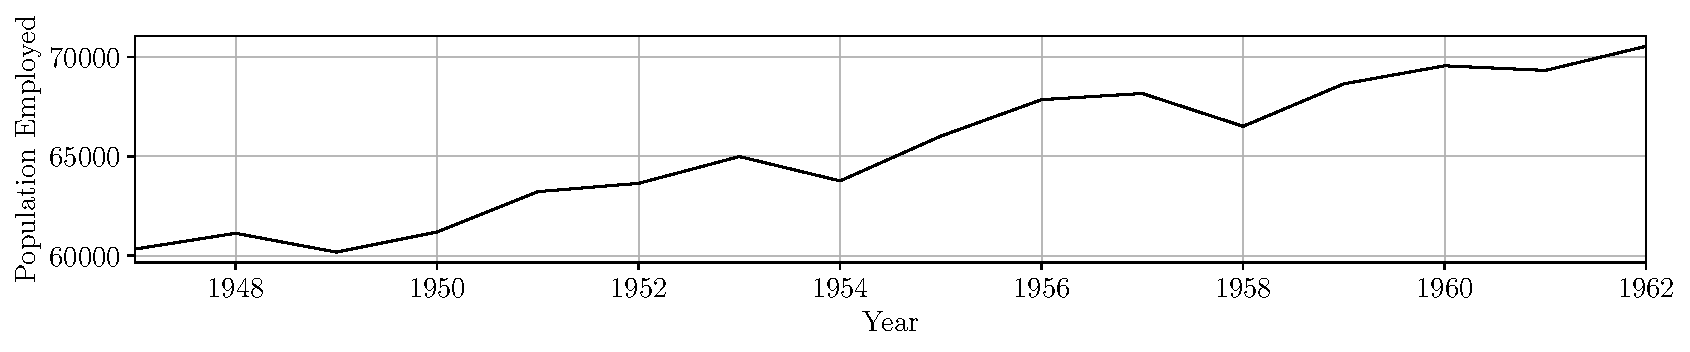
\includegraphics[width=\textwidth]{longley}
    \caption{Exemplo de tendência.}
    \label{fig:trend}
\end{figure}

Padrões sazonais ocorrem quando um fenômeno observado é afetado por fatores
sazonais, por exemplo o período do ano ou a hora do dia, esse necessariamente
de uma frequência fixa conhecida
\cite{hyndman2018forecasting,brockwell2016introduction}. Na Figura
\ref{fig:seasonality}, é apresentado uma série de observações da temperatura
média diária na cidade de Melbourne, Austrália ao longo de 10 anos, essa séria
apresenta um padrão de sazonalidade, sendo a temperatura da terra afetada pelo
ciclo solar e as estações do ano, é possível observar a periodicidade do
aumento e diminuição da temperatura relacionado a isso.

\begin{figure}[ht]
    \centering
    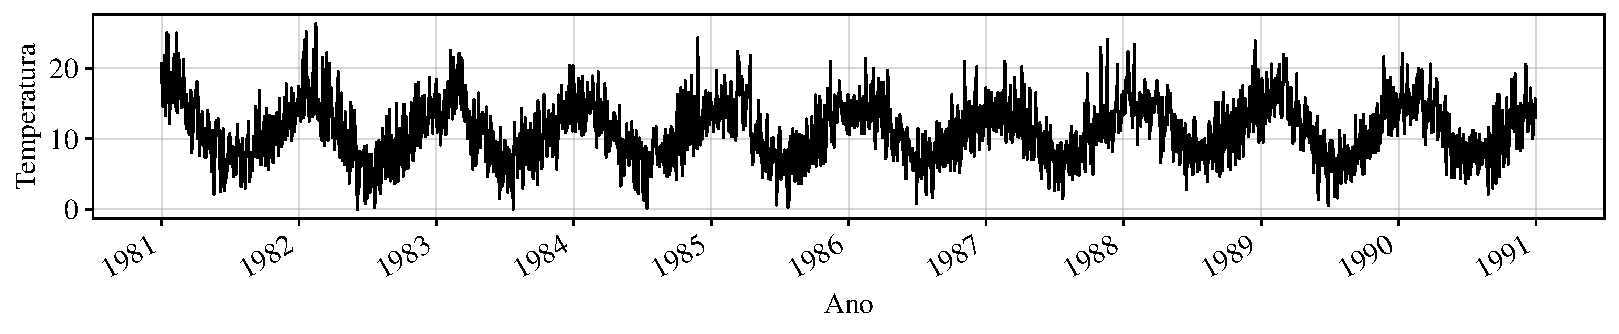
\includegraphics[width=\textwidth]{temperature}
    \caption{Exemplo de sazonalidade.}
    \label{fig:seasonality}
\end{figure}

Já mudanças de conceito, diferente de tendência ou sazonalidade em que média e variância são alteradas por um movimento claro, na mudança de conceito há uma quebra abrupta entre essas medidas estatísticas ao longo do tempo. Na Figura \ref{fig:concept_drift}, pode ser observado esse fenômeno, em que na altura do ponto 1000 a uma quebra da volatilidade observada anteriormente.

\begin{figure}[ht]
    \centering
    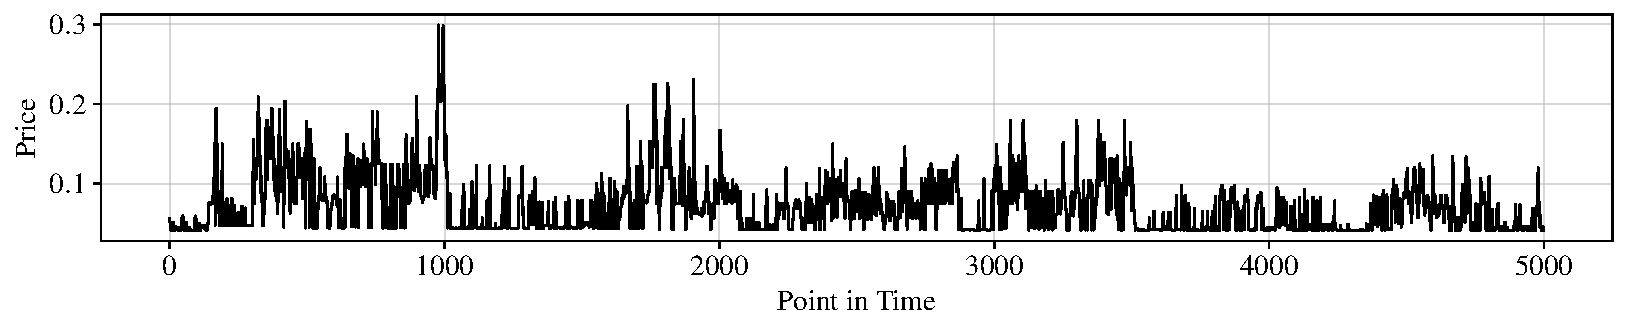
\includegraphics[width=\textwidth]{elec}
    \caption{Exemplo de mudança de conceito.}
    \label{fig:concept_drift}
\end{figure}

A maioria das técnicas de AM assumem que os dados são independentes e
identicamente distribuídos (\textit{i.i.d.}), mas essas premissas geralmente não
se sustentam em ambientes de FD, como apontado por A. Bifet and R.
Gavald\`a (2007) \cite{bifet2007learning}, tendo em vista que os dados chegam
interminavelmente, é esperado uma evolução no processo gerador dos dados e, por isso, dependência temporal e mudanças de conceito podem ocorrer.  Outro aspecto critico é a imposição de limites
computacionais a esses ambientes, como memória, CPU, e largura de banda
\cite{bifet2010moa, gama2012survey}. Para resolver esses problemas, diversas
abordagens foram desenvolvidas, dentre elas, as mais proeminentes são
mecanismos de esquecimento, testes estatísticos e algoritmos adaptativos.

\section{Trabalhos Relacionados}



Mecanismos de esquecimento fazem dados recentes tornarem-se mais relevantes e
dados passados menos, um exemplo bastante adotado desse mecanismo são janelas deslizantes
\cite{gaber2005mining}, janelas deslizantes é um método agnóstico de modelo que passa lotes de dados, a cada iteração, removendo amostras muito antigas e substituindo-as por amostras mais recentes. Já sistemas baseados em testes estatísticos agem monitorando uma métrica
pre-definida, tal como performance preditiva do modelo (e.g. acurácia), e então ``disparam'' um
alarme quando a qualidade dessas métricas está abaixo de algum limiar
tolerável, demandando alguma ação para corrigir essa deterioração.

Exemplos dessa abordagem são o teste de Page-Hinkley e o \textit{Statistical
Process Control} \cite{gama2010knowledge}.
Baseado nessas duas soluções, janelas deslizantes e testes estatísticos, o \textit{ADaptive WINdowing} (ADWIN) \cite{bifet2007learning} usa testes para definir o tamanho de cada janela, ajustando ao ``tamanho do conceito''.
Entretanto, embora esses métodos sejam capazes de alarmar uma redução na performance dos modelos e adaptar o tamanho da janela a isso, não é possível identificar os algoritmos ou modelos que se tornaram mais apropriados ao novo conjunto de dados que está sendo gerado.

Algoritmos de aprendizado adaptativo, como o VFDT \cite{domingos2000mining},
foram inicialmente introduzidos com FD em mente, desempenhando aprendizado online e baixo consumo de memoria. Porém, não conseguiam se adaptar a mudança de conceito, um problema já conhecido na época.
Mais tarde, aprimoramentos foram propostos, como o CVFDT (um aprimoramento direto sobre o VFDT) \cite{hulten2001mining}, o HAT \cite{bifet2009adaptive} e o ARF \cite{gomes2017adaptive}, que podem lidar com variação de conceito aplicando janelas deslizantes sobre o processo de treinamento.
Entretanto, embora esses métodos esqueçam mais severamente dados passados quando ocorrer uma mudança de conceito, eles mantêm um espaço de hipótese fixo (Árvore de Decisão, para a maioria deles) para seleção em qualquer conceito que venha a surgir, logo, para conceitos distintos Árvores de Decisão podem não performar uma seleção ideal, gerando performances indesejáveis em algumas aplicações.

Diferente das abordagens descritas acima, o MetaStream trata essas limitações da seguinte forma: (i) esse framework não precisa manter um sistema de alarme quanto a performance do algoritmo preditivo, pois dado um conjunto de algoritmos de desempenho razoável a nível base, é esperado que o método costume selecione o melhor ao longo do tempo, sem que nunca atinja, de forma prolongada, baixa performance; (ii) é flexível quanto ao viés indutivo, pois, diferente dos algoritmos anteriormente listados, que são limitados a Árvores de Decisão, a nível base qualquer algoritmo adequado a tarefa pode ser usado, como SVMs, Processos Gaussianos, modelos lineares, entre outros, já que é almejando espaços de hipótese como tarefas de aprendizado \cite{rossi2014metastream}.

